\chapter{Despliegue de la aplicación}
\label{sec:cap6}
En la etapa de despliegue es cuando el software queda disponible para el uso y disfrute de
los usuarios. Supone una etapa fundamental para dar por finalizada la construcción del
software. 

A la hora de elegir un modelo de entorno cloud tenemos distintos modelos de cloud
computing, dependiendo de las partes de la infraestructura local que queramos gestionar.

\FloatBarrier
\begin{figure}[h]
	\centering	
	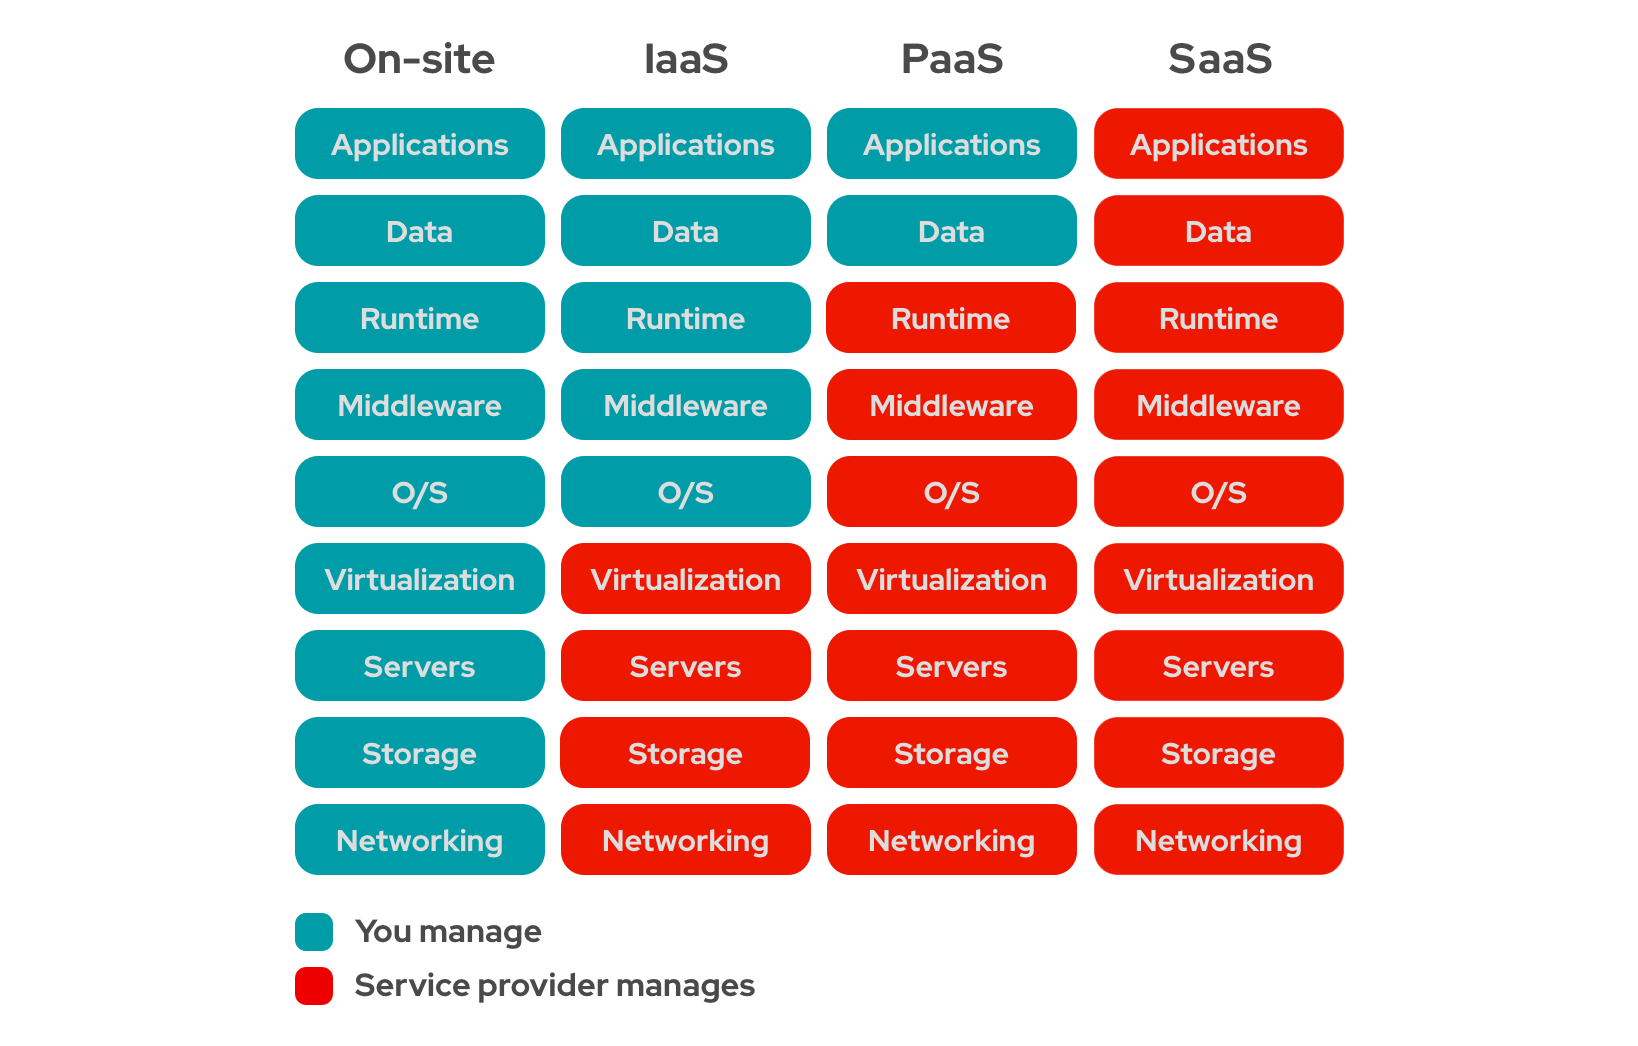
\includegraphics[width=\textwidth]{doc/logos/imgs/iaas-paas.png}
    \caption{ Distintos modelos de computación en la nube.
	\href{https://www.redhat.com/es/topics/cloud-computing/iaas-vs-paas-vs-saas}{RedHat -
	CC}}
    \label{fig:tipos-de-cc}
\end{figure}
\FloatBarrier


Necesito que el modelo de computación en la nube me provea de facilidad suficiente para
añadir y desplegar nueva funcionalidad con rapidez. El coste tiene que ser lo más
inteligente y adaptado posible. Y además, quiero un sistema que me prevea de una
plataforma ya estructurada de forma que solo tenga que centrarme en la configuración
correcta de mi servidor de acorde con los requisitos de la plataforma sin tener que
configurar ninguna infraestructura de bajo nivel como los puertos del sistema, el sistema
operativo\ldots


Estos requisitos hacen que utilizar como entorno cloud un PaaS, \textit{Platform as a
service} sea la mejor opción. Este me proveerá de varias capas de servicios apilados que me va a permitir ejecutar y
gestionar mi aplicación desplegada sin tener que mantener la infraestructura subyacente.


En el mercado existen distintas empresas que nos ofrecen este tipo de servicios, podemos
destacar: \href{https://aws.amazon.com/es/elasticbeanstalk/}{AWS Elastic Beanstalk},
\href{https://dashboard.heroku.com/login}{Heroku} o \href{https://vercel.com/}{Vercel}
entre otros. Mientras que Vercel no soporta (por el momento) despliegues basados en imágenes de docker,
que es la \hyperref[sec:proceso-despliegue]{forma de despliegue que persigo}, y AWS
solicita información bancaria, he utilizado Heroku.

\section{Proceso de despliegue}
\label{sec:proceso-despliegue}
Para poder desplegar una aplicación en Heroku, es necesario acceder al panel de
administración y crearnos una app. Sin embargo, existe un CLI \footnote{Interfaz de
línea de comandos} que se instala en nuestro sistema y nos permite realizar de forma más
cómoda las configuraciones necesarias.

A la hora de desplegar el código, Heroku nos ofrece distintas formas, una de ellas es
poner a la escucha una rama del repositorio de GitHub a cualquier tipo de cambio para
desplegarlo. Sin embargo, este proyecto tiene muchos \textit{assets}, los ficheros con
los datos de las defunciones que no están versionados en GitHub. Este
motivo y el poco margen de personalización que provoca este método sobre la
configuración de nuestra aplicación me hizo desestimar esta forma.

El método que he seguido ha sido crear un contenedor de la aplicación que luego publicamos
en la app creada en Heroku. Los contenedores, entre otras cosas, nos ofrecen tener una portabilidad absoluta
ya que podemos poner en marcha la aplicación en cualquier sistema operativo sin
preocuparnos de las dependencias necesarias y eso es lo que necesitamos hacer en el
servidor de Heroku.

El contenedor y su configuración se define como código en un archivo de texto plano
llamado \codeword{Dockerfile} en él se define el software necesario a instalar, las
dependencias del proyecto, se expone el host, el puerto y el número de \textit{workers}
\footnote{Son el número de procesos que va a ejecutar el dyno. En la versión gratuita de Heroku solo aprovechamos 2 \textit{workers} por
limitación del hardware.} a
ejecutar como variables de entorno que me permitirán a través del PaaS configurar o cambiar.
Por último, se especifica en el comando que ejecuta el contenedor.

\FloatBarrier
\begin{figure}[h]
	\centering	
	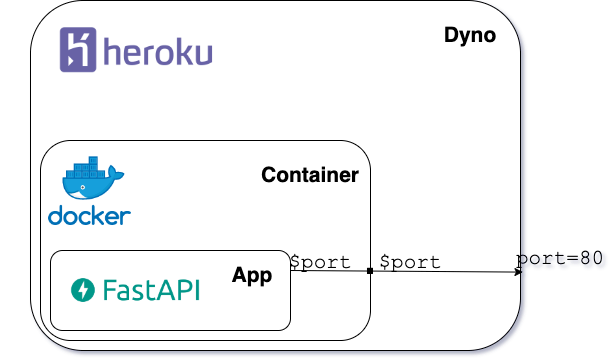
\includegraphics[width=\textwidth]{doc/logos/imgs/deployd.png}
	\caption{ Arquitectura del despliegue. }
    \label{fig:arq-deploy}
\end{figure}
\FloatBarrier

\begin{itemize}
    \item \textit{Dyno} es un contenedor liviano con Linux en los que Heroku ejecuta la
    aplicación.
\end{itemize}

Utilizando la CLI podemos ver el sistema de registros (que también está disponible en el
\textit{dashboard} web) con el que podemos monitorizar todas las peticiones que se
realizan así como los reinicios de la máquina virtual y el estado del servidor.

\FloatBarrier
\begin{figure}[h]
	\centering	
	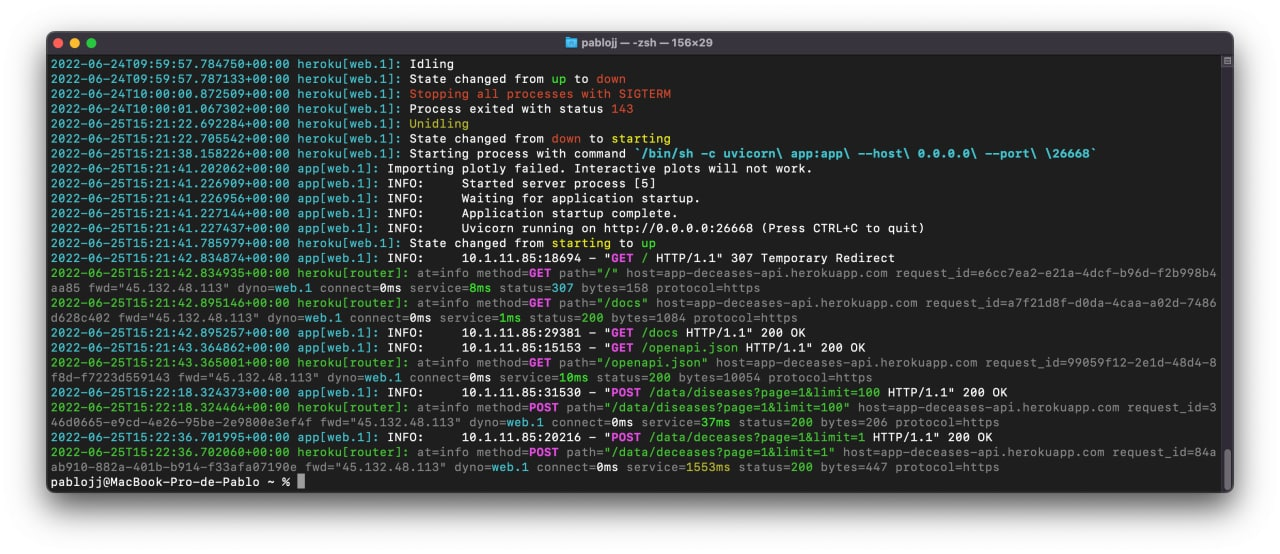
\includegraphics[width=\textwidth]{doc/logos/imgs/logs.jpg}
	\caption{ \textit{Logs} de la aplicación desplegada. }
    \label{fig:heroku-logs}
\end{figure}
\FloatBarrier

\section{Coste del despliegue}
\label{sec:despliegue}

Durante el proceso de desarrollo y las primeras pruebas se ha utilizado la modalidad ``Free
\& Hobby'' que nos permite desplegar la aplicación de forma gratuita con la limitación de
que la máquina entra en estado de reposo tras 30 minutos de inactividad, lo que
hace que cuando se reciba cualquier petición se encienda la máquina virtual que contiene
el contenedor con la aplicación, además los dynos \footnote{Es un contenedor liviano con Linux en los que Heroku ejecuta la
aplicación.}
tienen 2 cores por lo que nos limita el número de procesos.

Para la puesta en producción se debería de contratar la tarifa ``Standard 1X'' que nos ofrece
512MB de RAM, con ilimitado número de procesos gracias al autoescalada y nos incluye un
sistema de métricas y avisos que no está disponible en la versión gratuita. Esta tarifa
tiene un coste de 25\$ al mes.
